% !TeX root = ../thuthesis-example.tex

\chapter{模型建立}

针对一项高附加值化学分子产品的合成过程概念设计,通过对多种在实验室或小试规模下具有转化率、高选择性、高反应效率、原料易得性、低能耗、环境友好性等开发潜力的合成步骤、路径或单步工艺进行流程综合与过程设计是产品开发与市场预期的必经之路。综合考虑物料、设备与操作可行性,对于各种不同的合成路径组合进行筛选优化,可以起到良好的降低损耗、控制成本的作用,同时便于全流程自动化控制系统的研究,因此在药物研发与工艺开发中应当重视并增加运用\cite{mencarelli2020,matsunami2020}。基于此,本章将对通过已有文献整理的来自文献、专利与有机化学工艺库中的507条三步连续合成卢非酰胺的路径建立合成路径超结构优化模型,包括综合考虑固定投资和操作成本等多个构成要素在内的生产成本预估函数和计算利用流动微反应器设计连续合成过程的产能与设备数量的数学规划模型。在对确定性模型开展灵敏度分析之后,结合生产过程常面临的不确定因素,确定了生产目标、生产时间与公用工程费用三个不确定因素作为不确定性分析和优化的抓手。为了让设计具有完全应对不确定性的能力,借鉴两阶段ARO方法,将第一阶段变量设置为路径决策变量,第二阶段变量即追索变量设置为设计变量,构造了不确定条件下的卢非酰胺连续合成优化设计模型。

\section{卢非酰胺合成过程}

卢非酰胺的三步合成方法在有机化学领域具有一定代表性,因此已经有研究工作者对各个合成步骤的路径与工艺进行了整理和扩充性质的工作\cite{padmaja2018}。虽然报道的工作中各个合成路径都有方法与效果上的创新与优势,但是,在特定生产场景下的连续合成路径组合选取存在着优势和劣势的竞争,例如无溶剂合成(Solvent-free Synthesis)工艺虽然降低了溶剂的消耗,减轻了环境影响,但在连续流动反应装置中限制了流速从而可能限制生产规模,如果增加同步设备又可能提高综合成本\cite{gelonch2019};同理,基于填充催化剂的部分反应可能导致操作与物料成本的增长,诸如此类。因此,超结构优化是最佳的总体衡量各方面因素的概念设计方法。

\begin{figure}
  \centering
  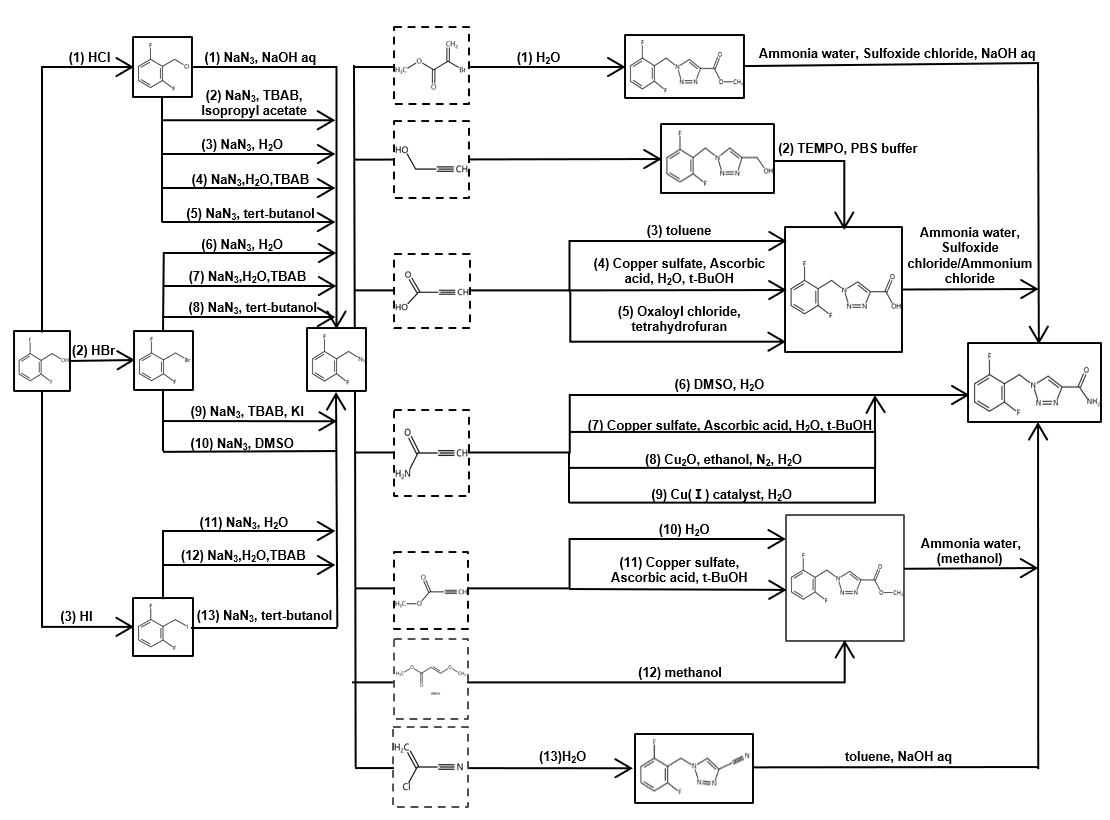
\includegraphics[width=1.1\linewidth]{superstructure1.png}
  \caption*{超结构示意图中的节点即边内的虚线框分别是合成主要物料的结构式,每条边对应一种具体合成路径}
  \caption{超结构模型示意图}
  \label{fig:superstructure}
\end{figure}

对于第一步卤化反应,在数据整理过程中我们发现针对三种主流卤化试剂(氯化氢、溴化氢、碘化氢)均有经过工艺研发者优化的合适的反应条件,且可以适用于连续反应,因此为了降低模型中不必要的复杂度,我们使用了一处贪心策略,在第一步中已经选取了各方面工艺参数都局部最优的三条路径纳入超结构中。值得注意的是,每种卤化试剂都选取了一条备择路径,无论优化决策结果如何,这并不代表其他试剂选择不存在拥有更优的合成路径的可能。这是由于缺乏足够的实验数据和机理模拟的手段,本工作在概念设计阶段无法直接对单步反应工艺在开发源头进行优化。

第二步叠氮化反应对第一步底物的适应性均较好,只是在最优操作条件方面有出入,在该步骤我们选取了所有可能的工艺组合共13种。本步骤中各工艺在溶剂选择方面存在较大差异,因此对反应体系的温度需求、操作需求和设备选型有一定影响。反应完成之后存在一步控温连续萃取操作,由于目标产物相同,该操作未包含在超结构内,但是纳入了对结构选型的优化的考量中。

第三步通过叠氮参与的1,3-偶极环加成反应生成相应的最终产物或前驱体,由于环加成反应过程中的极性中心处于优势区位,因此通常可以与亲核水解胺化等反应串联或一锅进行,是常见的有机连续合成策略。针对环加成过程,有两种反应机理,分别对应炔烃和烯醇类似底物,后者包含N-O的次级轨道相互作用,增强了烯醇类似底物的化学活性,因此拓展了反应的搜索空间\cite{paz2018}。图\ref{fig:superstructure}中对第三步反应的转化过程做了更详细的展示,共13种纳入考虑的合成路径。第三步中涉及的各个反应工艺的定制化都较强,在模型的数据准备中分别做了相应的考虑和计算,这为超结构模型的建立带来了形式上的统一。

\section{模型优化目标及约束}
\subsection{模型假设}

在建立超结构设计模型时,本文做出如下假设,在不失模型效力和不违背生产规律的前提下帮助模型尽可能得到有益的简化。

第一,假设各种所需物料的价格是定值,在生产过程中可以稳定获取不发生波动。本条假设是在调研了相关化学品近年的市场价格变动情况与数据丰富程度之后做出的。

第二,针对任一生产路径,不核算上游原材料及所有涉及物流的运输及仓储成本。

第三,假设所有超结构包含的合成路径在生产技术条件上是可行的,即未考虑由于工厂选址、地区因素,政策或环境因素引起的不支持特定操作要求和生产安排的情况,且生产装置在建设时已经充分考虑到为不确定性实现预留的操作空间。

第四,假设各生产路径的反应转化率是定值。本条假设要求反应条件在生产过程中的精准控制,应对催化剂更换或设备检修的详尽计划,由于这些工作是在概念设计阶段之后开展的,本文暂不考虑。

第五,假设使用的管式流动微反应器是完美数量放大的。本条假设要求所有的流动微反应器在制造和操作条件控制方面达到一致,因此产能可以呈整数倍数进行放大。这在设计阶段是合理的,并由此产生了追索问题的混合整数设计变量。

第六,对于固定投资的计算,假设其与设备操作量(对于本模型中通常按操作容积计)成正比,并按照设备购进价格按折旧率折算年费。

第七,对于操作成本的计算,假设公用工程费用以设计变量和参数的线性函数折算,对于能量消耗项的估算,认为与操作温度和室温的差成正比。

\subsection{成本函数}

如前所述,卢非酰胺的合成超结构优化主要以生产成本核算为优化目标。经济评估的目标往往是多方面的,为了模型的简明性和可解释性,在化工过程的概念设计过程中往往应用线性加合的方式构造单目标的成本函数\cite{yeoman1999,gong2017,madenoor2018},本模型的成本主要考虑选择相应工艺组合的年平均生产成本,包括以下各个部分。

第一,物料成本(Material Expenditure, $\symbfup{ME}$),如式\eqref{eq:me}。首先通过化学品交易平台数据库等获取,价格以美元计算;然后根据物料种类不同进行数据处理,具体而言,对于有明确投料比的合成原料或助剂,按照生产单位摩尔产物折算价格因子$c$;对于催化剂或可循环溶剂等,按照文献推测的更换频率,同样折算为生产单位摩尔产物的价格;对于一般的流动载体介质考虑在操作成本的溶剂回收项中。
\begin{align}
  \symbfup{ME} = \frac{\sum_{s}\symbfit c_s^T\symbfit X_s}{M_{\rm ruf}} \label{eq:me}
\end{align}
其中$s$为合成步骤的集合下标。

第二,固定成本(Capital Expenditure,$\symbfup{CE}$),如式\eqref{eq:ce}。固定成本投资只考虑了微反应器设备组件的资产投入\cite{diab2018,borukhova2016},按照连续药物分子合成工业设计的惯例,采用了按照标准设备投资($CE_0=374,600$美元)乘以容积因子\cite{diab2019}的方法估算。年费折旧率当开工时间$\symbfit\tau$不小于7000小时时按照全年8000小时计算,小于7000小时时按照近似的经验公式$\epsilon=15\%\times(1-\frac{\symbfit\tau}{8000})^{0.5}$计算\cite{baasal1989}。
\begin{align}
  \symbfup{CE} = \frac{\epsilon CE_0}{80.00}\sum_{s}\symbfit N_s\symbfit V_s \label{eq:ce}
\end{align}
其中$\symbfit N_s$表示设备台数,$\symbfit V_s$代表操作容积。

第三,操作成本(Operational Expenditure,$\symbfup{OE}$),如式\eqref{eq:oe}。操作成本项考虑了溶剂分离和处理操作的成本与电加热设备的能量消耗对应的公用工程支出,此处我们参考\cite{diab2018}的工作,按照系数折算法\cite{garrett2012}对两项成本进行估算,目的是为了考虑各个路径工艺选择在操作成本上的影响,以达到综合经济与环境因素影响的评估。
\begin{align}
  \symbfup{OE} = \sum_s \big(\xi\symbfit\tau_s(T_s-T_0)\symbfit N_s\symbfit L_s +E_{\rm rec}(1-r_{rec})\symbfit N_s\symbfit L_s\symbfit V_s\big) \label{eq:oe}
\end{align}
其中各参数符号含义见表\ref{tab:notation},详细的计算方法在\ref{section:shebei}节中阐述。

\subsection{物料守恒}

引入变量$\symbfit X_s$对各个生产步骤的产能(即一年时间内该步主产物的总摩尔流量)进行描述,因此涉及到对每步步骤间的转化率进行核算,转化率采用基于上步产物纯品投料为基准计算,由于涉及到单程转化率、产率、分离比率等工艺细节问题,在物料衡算方面每步用统一的$\symbfit r_s$描述最终转化为该步产物纯品的表观产率,然后根据文献对工艺开发的描述和计算推测,根据单程转化时间$\symbfit \tau_s$的大小来反映若选择性和转化率低导致的额外分离对生产效能的影响。最终,第三步反应结束的后的产品卢非酰胺的目标用$PT$,以质量计的年生产目标这一超参数来约束。基于以上建模手段,物料守恒的约束为式\eqref{eq:mb1}-\eqref{eq:mb2}。
\begin{align}
  \symbfit X_0\sum_{i\in\mathbb I}\symbfit Y_i\symbfit r_i&=\sum_{i\in\mathbb I}\symbfit X_i \label{eq:mb1} \\
  \sum_{i\in\mathbb I}\symbfit X_i\sum_{j\in\mathbb J}\symbfit Y_j\symbfit r_j&=\sum_{j\in\mathbb J}\symbfit X_j \\
  \sum_{j\in\mathbb J}\symbfit X_j\sum_{k\in\mathbb K}\symbfit Y_k\symbfit r_k&=\sum_{i\in\mathbb K}\symbfit X_k \\
  \sum_{k\in\mathbb K}\symbfit X_kM_{\rm ruf}&\ge PT \label{eq:mb2}
\end{align}

\subsection{设备设计}
\label{section:shebei}

\section{逻辑约束}

超结构优化中的逻辑约束通常引入与决策维度相关的二元变量向量或矩阵来描述,最直观的一种表述就是“某个选项被选中/不被选中”分别对应二元变量“$\symbfit Y=1$/$\symbfit Y=0$”。对于本文模型,由于不需要类似STN网络中涉及多个任务类型的选取和转化,而是结构化地选取各步骤工艺路径,因此逻辑约束相对简单,如式\eqref{eq:lc1}-\eqref{eq:lc2}。其中$\symbfup M=10^5$为一个足够大的常量
\begin{align}
  \sum_{i\in\mathbb I}\symbfit Y_i&=1 \label{eq:lc1} \\
  \sum_{j\in\mathbb J}\symbfit Y_j&=1 \\ 
  \sum_{k\in\mathbb K}\symbfit Y_k&=1 \\
  \symbfit X_s &\le \symbfup M\symbfit Y_s,\ \forall s\in \mathbb S = \mathbb I \cup\mathbb J\cup\mathbb K \label{eq:lc2} 
\end{align}

\section{确定性模型评估}
\subsection{确定性模型}

\begin{longtable}{cc}
  \caption{本文超结构优化模型的符号释义表}
  \label{tab:notation} \\
  \toprule
  参数或变量符号 & 含义 \\
  \midrule
\endfirsthead
  \caption*{续表~\thetable\quad 本文超结构优化模型的符号释义表} \\
  \toprule
  参数或变量符号 & 含义 \\
  \midrule
\endhead
  \bottomrule
\endfoot
Row 1  & & & \\
Row 2  & & & \\
Row 3  & & & \\
Row 4  & & & \\
Row 5  & & & \\
Row 6  & & & \\
Row 7  & & & \\
Row 8  & & & \\
Row 9  & & & \\
Row 10 & & & \\
\end{longtable}

\subsection{确定性模型求解结果}

\section{不确定性优化模型}
\subsection{灵敏度分析与不确定参数选取}
\subsection{鲁棒优化模型}
\subsection{两阶段ARO模型建立}


\section{插图}

图片通常在 \env{figure} 环境中使用 \cs{includegraphics} 插入,如图~\ref{fig:example} 的源代码。
建议矢量图片使用 PDF 格式,比如数据可视化的绘图;
照片应使用 JPG 格式;
其他的栅格图应使用无损的 PNG 格式。
注意,LaTeX 不支持 TIFF 格式;EPS 格式已经过时。

\begin{figure}
  \centering
  
\includegraphics[width=0.5\linewidth]{example-image-a.pdf}
  \caption*{国外的期刊习惯将图表的标题和说明文字写成一段,需要改写为标题只含图表的名称,其他说明文字以注释方式写在图表下方,或者写在正文中。}
  \caption{示例图片标题}
  \label{fig:example}
\end{figure}

若图或表中有附注,采用英文小写字母顺序编号,附注写在图或表的下方。
国外的期刊习惯将图表的标题和说明文字写成一段,需要改写为标题只含图表的名称,其他说明文字以注释方式写在图表下方,或者写在正文中。

如果一个图由两个或两个以上分图组成时,各分图分别以 (a)、(b)、(c)...... 作为图序,并须有分图题。
推荐使用 \pkg{subcaption} 宏包来处理, 比如图~\ref{fig:subfig-a} 和图~\ref{fig:subfig-b}。

\begin{figure}
  \centering
  \subcaptionbox{分图 A\label{fig:subfig-a}}
    {
\includegraphics[width=0.35\linewidth]{example-image-a.pdf}}
  \subcaptionbox{分图 B\label{fig:subfig-b}}
    {
\includegraphics[width=0.35\linewidth]{example-image-b.pdf}}
  \caption{多个分图的示例}
  \label{fig:multi-image}
\end{figure}



\section{表格}

表应具有自明性。为使表格简洁易读,尽可能采用三线表,如表~\ref{tab:three-line}。
三条线可以使用 \pkg{booktabs} 宏包提供的命令生成。

\begin{table}
  \centering
  \caption{三线表示例}
  \begin{tabular}{ll}
    \toprule
    文件名          & 描述                         \\
    \midrule
    thuthesis.dtx   & 模板的源文件,包括文档和注释 \\
    thuthesis.cls   & 模板文件                     \\
    thuthesis-*.bst & BibTeX 参考文献表样式文件    \\
    \bottomrule
  \end{tabular}
  \label{tab:three-line}
\end{table}

表格如果有附注,尤其是需要在表格中进行标注时,可以使用 \pkg{threeparttable} 宏包。
研究生要求使用英文小写字母 a、b、c……顺序编号,本科生使用圈码 ①、②、③……编号。

\begin{table}
  \centering
  \begin{threeparttable}[c]
    \caption{带附注的表格示例}
    \label{tab:three-part-table}
    \begin{tabular}{ll}
      \toprule
      文件名                 & 描述                         \\
      \midrule
      thuthesis.dtx\tnote{a} & 模板的源文件,包括文档和注释 \\
      thuthesis.cls\tnote{b} & 模板文件                     \\
      thuthesis-*.bst        & BibTeX 参考文献表样式文件    \\
      \bottomrule
    \end{tabular}
    \begin{tablenotes}
      \item [a] 可以通过 xelatex 编译生成模板的使用说明文档;
        使用 xetex 编译 \file{thuthesis.ins} 时则会从 \file{.dtx} 中去除掉文档和注释,得到精简的 \file{.cls} 文件。
      \item [b] 更新模板时,一定要记得编译生成 \file{.cls} 文件,否则编译论文时载入的依然是旧版的模板。
    \end{tablenotes}
  \end{threeparttable}
\end{table}

如某个表需要转页接排,可以使用 \pkg{longtable} 宏包,需要在随后的各页上重复表的编号。
编号后跟表题(可省略)和“(续)”,置于表上方。续表均应重复表头。

\begin{longtable}{cccc}
    \caption{跨页长表格的表题}
    \label{tab:longtable} \\
    \toprule
    表头 1 & 表头 2 & 表头 3 & 表头 4 \\
    \midrule
  \endfirsthead
    \caption*{续表~\thetable\quad 跨页长表格的表题} \\
    \toprule
    表头 1 & 表头 2 & 表头 3 & 表头 4 \\
    \midrule
  \endhead
    \bottomrule
  \endfoot
  Row 1  & & & \\
  Row 2  & & & \\
  Row 3  & & & \\
  Row 4  & & & \\
  Row 5  & & & \\
  Row 6  & & & \\
  Row 7  & & & \\
  Row 8  & & & \\
  Row 9  & & & \\
  Row 10 & & & \\
\end{longtable}



\section{算法}

算法环境可以使用 \pkg{algorithms} 或者 \pkg{algorithm2e} 宏包。

\renewcommand{\algorithmicrequire}{\textbf{输入:}\unskip}
\renewcommand{\algorithmicensure}{\textbf{输出:}\unskip}

\begin{algorithm}
  \caption{Calculate $y = x^n$}
  \label{alg1}
  \small
  \begin{algorithmic}
    \REQUIRE $n \geq 0$
    \ENSURE $y = x^n$

    \STATE $y \leftarrow 1$
    \STATE $X \leftarrow x$
    \STATE $N \leftarrow n$

    \WHILE{$N \neq 0$}
      \IF{$N$ is even}
        \STATE $X \leftarrow X \times X$
        \STATE $N \leftarrow N / 2$
      \ELSE[$N$ is odd]
        \STATE $y \leftarrow y \times X$
        \STATE $N \leftarrow N - 1$
      \ENDIF
    \ENDWHILE
  \end{algorithmic}
\end{algorithm}
